% MAP paper -- ACM acmart, sigconf, preprint (nonacm).
% Build: latexmk -pdf main.tex   (or upload the paper/ directory to Overleaf)
% Every number in this paper comes from eval/results/5bc7702/ (REPORT.md, B2L.md,
% MINIMAX.md) or from the repository at the tag cited in Appendix A.
\documentclass[sigconf,nonacm]{acmart}

\settopmatter{printacmref=false, printfolios=true}
\renewcommand\footnotetextcopyrightpermission[1]{}
\pagestyle{plain}

\usepackage{multirow}

\newcommand{\sys}{MAP}
\newcommand{\eg}{e.g.,\ }
\newcommand{\ie}{i.e.,\ }
\newcommand{\ci}[2]{\,[#1,\,#2]}
\newcommand{\hyp}[1]{\textsf{#1}}

\begin{document}

\title{Mutual Attestation for Delegated Agent Work}
\subtitle{Dual-Signed Evidence, Observer-Local Trust, and Countersigned Resumption over A2A}

\author{Jesse Larsen}
% TODO(author): set \country{...}; acmart warns when it is missing.
\affiliation{\institution{Independent researcher}\country{}}
\email{jesselarsen@gmail.com}

\begin{abstract}
When one AI agent delegates work to another, three questions follow: did
the work happen as claimed, whom to trust next time, and can another
worker take over after a failure without the delegator paying twice or
trusting the failed worker's word? A2A carries the task but leaves these
questions open. We present \sys{}, a thin accountability layer over A2A,
a Kademlia discovery index and existing payment rails. Only a receipt
signed by \emph{both} parties counts as positive evidence. Each observer
computes trust locally from receipts it can verify, weighting other
issuers by how well they agree with its own experience. The requester
countersigns transcript checkpoints, so a task can resume on another
provider and a failed provider can bill only for acknowledged work. Rust
and Go implementations interoperate with each other and with an
unmodified A2A SDK client.
We evaluate \sys{} against pre-registered hypotheses, after replicating a
recent agent P2P simulation to within 0.024. The main trust hypothesis is
only partially supported, holding in 18 of 28 settings. It predicted that
local trust, with our pre-registered weighting, at least halves the
attacker share of both a global ledger and a canary-only baseline, over
seven attacks at adversarial fractions up to 0.3.
A global ledger collapses under slander (0.95 attacker share at
$\alpha{=}0.5$); local trust does not (0.08). In an exploratory
comparison, \sys{} with a canary beats the replicated work's
canary-plus-ledger design in 25 of 35 settings and ties in 10.
Countersigned resumption wastes 0.42\% of the work restarting does.
\sys{} loses during cold start; to a global ledger under on-off,
whitewashing and camouflage; without a canary, to the canary-plus-ledger
design under whitewashing and slander; and, with our pre-registered
weighting, under Sybil-majority camouflage, which changed the recommended
default. Identifier grinding remains unmitigated.
\end{abstract}

\keywords{AI agents, accountability, reputation, Sybil resistance, A2A,
checkpointing, verifiable receipts}

\maketitle

\section{Introduction}
\label{sec:intro}

Agents increasingly delegate work to other agents they do not operate.
A planning agent sends a translation subtask to a provider it found in a
directory. A coding agent rents inference from whichever peer has capacity.
Protocols for this exchange have matured quickly. A2A~\cite{a2a2026}
reached version~1.0 in March 2026 with signed Agent Cards. Directory
services index agents by capability~\cite{ads2026,nanda2025}. Payment
rails meter usage with payer-signed cumulative
vouchers~\cite{mpp2026,x402v2}. What these protocols do not provide is
\emph{accountability} for the delegated work itself. Three questions stay
open:

\begin{enumerate}
\item \textbf{Evidence.} After a task, what record exists that both sides
  can rely on? A provider-signed receipt shows what the provider
  \emph{claims} it did. The requester can dispute it but cannot disprove
  it.
\item \textbf{Trust.} When choosing a provider, whose opinion counts? A
  global ledger aggregates every issuer's feedback. On-chain, that
  aggregate is dominated by coordinated Sybils: 59--91\% of reviewers in
  the ERC-8004 reputation registry show coordinated Sybil
  behaviour~\cite{xiong2026erc8004}.
\item \textbf{Failure.} If the provider dies halfway through a long task,
  can another provider continue, and on whose word about progress? If the
  resumption point is the failed provider's own claim, the failed provider
  can overbill, and the successor inherits a transcript nobody verified.
\end{enumerate}

Wang et al.\ recently argued that agent networks generalize peer-to-peer
file sharing from ``who has this file?'' to ``who can do this
task?''~\cite{wang2026agenticp2p}. Their system uses signed capability
descriptors, provider-signed receipts, and a local plus federated
reputation ledger. It is evaluated in simulation. We build on that framing
and ask what the \emph{accountability} layer of such a network must look
like if it is to survive adversaries who can mint identities for free.

\paragraph{Approach.}
\sys{} (Mutual Attestation Protocol) is a thin layer that runs \emph{over}
existing systems rather than replacing them: A2A carries the task, a
Kademlia index carries discovery records, and MPP or x402 moves money.
\sys{} adds four things (\S\ref{sec:design}):
\begin{itemize}
\item \textbf{Dual-signed receipts} (\S\ref{sec:receipts}). Only a receipt
  countersigned by the requester can count \emph{for} a provider. A
  requester-only receipt can still count against one. This removes the
  provider's ability to manufacture positive evidence alone.
\item \textbf{Observer-local trust with a rebuild rule} (\S\ref{sec:trust}).
  Each observer computes trust from receipts it has verified. An issuer
  with no evidence relationship to the observer weighs zero, and the
  projection is a pure function of the receipt store.
\item \textbf{Countersigned checkpoints} (\S\ref{sec:checkpoints}). The
  requester countersigns a Merkle root over the transcript and the
  cumulative usage. For tasks whose state is their output stream, any
  provider can resume from that point after verifying the replayed
  prefix. A failed provider can bill only up to the last acknowledged
  checkpoint.
\item \textbf{Evidence-bound metering} (\S\ref{sec:metering}). Checkpoints
  and receipts carry a digest of the rail voucher that pays for the usage
  they record, without \sys{} defining a payment method.
\end{itemize}

\paragraph{Contributions.}
\begin{enumerate}
\item The design of \sys{} and a normative specification with an A2A~v1.0
  extension binding (\S\ref{sec:design}, \S\ref{sec:binding}).
\item Two implementations, in Rust and Go. They interoperate over A2A with
  each other (28/28 cells of a live interop matrix) and with an unmodified
  A2A Python SDK client. Along the way we found that the SDK's Agent Card
  canonicalization differs from the A2A specification's
  (\S\ref{sec:implementation}).
\item A pre-registered evaluation (\S\ref{sec:evaluation}). It reproduces
  Wang et al.'s published attack curve to within 0.024, measures \sys{}
  against a global ledger and a canary baseline under seven attacks, and
  quantifies checkpointed resumption, discovery attacks and metering
  overhead. We report every verdict, including failed ones. An
  exploratory comparison against the design Wang et al.\ describe, a
  canary plus a provider-signed ledger, shows \sys{} with a canary
  better in 25 of 35 settings, with overlapping CIs in the other 10. Without the canary, \sys{} is
  worse than that design under whitewashing and slander.
\item Measured confirmations of three known weaknesses in the agent
  setting. Two of them changed the specification: one the default
  weighting, and the other made epoch-salted sharding NOT RECOMMENDED as
  a mitigation
  (\S\ref{sec:eval-trust}, \S\ref{sec:eval-discovery}):
  \begin{itemize}
  \item a global ledger that admits unilateral complaints collapses under
    slander from free Sybils (0.95 attacker share at $\alpha{=}0.5$);
  \item trust propagation over an agreement graph collapses once
    camouflaging Sybils outnumber honest issuers, which is the scarce
    attack edges that graph-based Sybil defences assume
    away~\cite{yu2006sybilguard};
  \item epoch-salted shard assignment does not stop identifier grinding
    when identities are free~\cite{douceur2002sybil}.
  \end{itemize}
\item A methodological lesson. Our pre-registered rule for choosing the
  default weighting was applied at a single adversarial fraction, and the
  weighting it chose collapsed at a fraction the rule never examined. A
  minimax rule over the whole grid, pre-registered before its run,
  reversed the choice. A pre-registration should fix where a decision is
  tested, not only how it is made.
\end{enumerate}

\paragraph{What we do not claim.}
Dual-signed receipts are not new in themselves. TrustChain already uses
records signed by both parties as a Sybil defence~\cite{otte2020trustchain},
Signet's bilateral receipts co-sign MCP tool calls~\cite{signet}
(\S\ref{sec:related} compares them with \sys{}'s in detail), and
accountable distributed systems have long used signed, tamper-evident
logs~\cite{haeberlen2007peerreview}. Nor is agreement-weighted,
observer-local trust new~\cite{xiong2004peertrust,walsh2006credence}.
Our contribution is the combination for agent delegation, the countersigned
resumption, and the pre-registered measurement. \sys{} does not make agents honest.
It makes their claims attributable, and it lets each observer decide how
much evidence it needs. Identifier grinding and cold start remain open
(\S\ref{sec:limitations}).

\section{Background and Setting}
\label{sec:background}

\paragraph{Delegated agent work.}
A \emph{requester} agent delegates a task to a \emph{provider} agent.
The provider streams output as a sequence of \emph{Parts} and ends in a
terminal state: completed, failed or cancelled. The requester may pay per
unit of usage: tokens, milliseconds or invocations. Either party may be
adversarial. Identities are public keys that anyone can generate at no
cost.

\paragraph{A2A.}
A2A~v1.0~\cite{a2a2026} defines tasks, messages and artifacts over
JSON-RPC, REST and gRPC bindings. It defines an \emph{Agent Card} that
advertises an agent's skills and can be signed (JWS over a canonical JSON
form). Extensions are advertised in the card, activated per request with
an \texttt{A2A-Extensions} header, and may carry data in
\texttt{metadata} maps. A2A says nothing about evidence of execution,
reputation or resumption on another agent. Those are the parts \sys{}
supplies. MCP~\cite{mcp2025} connects an agent to its tools, not to other
agents. The IETF's proposed agentproto working group~\cite{agentproto2026}
targets common requirements for agent dialogs.

\paragraph{Discovery.}
The Agent Directory Service~\cite{ads2026} stores signed agent records
in a Kademlia DHT~\cite{maymounkov2002kademlia}, keyed by capability.
NANDA~\cite{nanda2025} proposes a lean index that resolves to
cryptographically verifiable ``AgentFacts''.

\paragraph{Metering rails.}
MPP's \emph{session} intent~\cite{mpp2026} and the batch-settlement scheme
of x402~V2~\cite{x402v2} both let a payer sign cumulative authorizations
as usage accrues, and pause delivery until the next one arrives. This
makes payment channels~\cite{poon2016lightning} practical for agent
metering. What the rail proves is that money moved or was authorized. It
does not prove which work that money bought, or that the work happened.

\paragraph{The baseline we build on.}
Wang et al.~\cite{wang2026agenticp2p} proposed ``Agentic P2P'' networks.
They also released a simulator (v0.3.10), which we re-implemented from
source for our replication (\S\ref{sec:eval-f1}). Reading that source, we
found two things:
\begin{itemize}
\item the trust value used for provider ranking is a hint the provider
  reports about itself;
\item the ``Risk-Aware'' policy is a memoryless per-task canary: it tests
  a candidate with a probe task before delegating, and falls back to
  another candidate on failure.
\end{itemize}
The paper's prose also describes a ``federated community ledger'' of
provider-signed receipts. Its simulator does not implement one. We
therefore model the ledger as a separate baseline (B2L).

\section{Threat Model and Goals}
\label{sec:threat}

\paragraph{Adversary.}
The adversary controls a fraction $\alpha$ of providers. It can create any
number of requester and provider identities at negligible cost (a key pair
costs about $16\,\mu$s on one core, \S\ref{sec:eval-discovery}). It can
collude across all of them, sign anything with keys it holds, publish
arbitrary receipts to any shared store, refuse to countersign, and change
behaviour over time. It controls a fraction $f$ of DHT routers and can
answer lookups arbitrarily. It cannot forge signatures of honest keys or
break SHA-256. We do not model network-level denial of service or
compromised honest keys. Key rotation and revocation are out of scope in
this version.

\paragraph{Attacks.}
We evaluate the classic reputation
attacks~\cite{hoffman2009survey,douceur2002sybil,feldman2006whitewashing},
instantiated for agent delegation:
\begin{itemize}
\item \emph{farming}: Sybil requesters issue positive receipts for their
  own providers;
\item \emph{camouflage}: farming Sybils also run truthful tasks against
  honest providers, to look like good raters;
\item \emph{collusion}: adversarial providers vouch for each other;
\item \emph{whitewashing}: adversarial providers re-enter under fresh
  identities;
\item \emph{on-off}: adversarial providers alternate good and bad
  phases;
\item \emph{slander}: Sybils file negative receipts against honest
  providers;
\item \emph{combined}: farming plus slander plus selective
  countersigning.
\end{itemize}
In discovery, the adversary attempts \emph{shard flooding} (publishing
records outside the shard they belong to), \emph{identifier grinding}
(generating identities until they land in a target shard), and
\emph{eclipse} of lookups through malicious routers.

\paragraph{Goals.}
\begin{description}
\item[G1 Attributability.] Positive evidence about a provider exists only
  if the requester agreed to it. Negative evidence is attributable to a
  requester.
\item[G2 Local soundness.] An observer's view of a provider depends only on
  receipts it can verify, weighted by its own policy. Evidence from
  issuers with no relationship to the observer contributes nothing.
\item[G3 Safe resumption.] A task resumes only from a state that the
  requester verified. A failed provider is owed at most the usage of its
  last countersigned checkpoint.
\item[G4 Bounded exposure.] Under voucher-per-checkpoint metering, neither
  side is exposed beyond one checkpoint interval of usage.
\item[G5 Composability.] Plain A2A clients keep working, and \sys{} adds
  no payment method, transport or task protocol of its own.
\end{description}
Confidentiality of task content is \emph{not} a goal. \sys{}'s
data-sensitivity zones are dual-signed labels with a refusal rule, which
provides accountability rather than confidentiality (\S\ref{sec:zones}).

\section{Design}
\label{sec:design}

\sys{} defines artifacts and rules, not a protocol stack.
Figure~\ref{fig:flow} shows how the artifacts ride on an A2A task.
Everything below is normative in the specification. We give its essential
content here and cite rule identifiers (\eg R-4) so readers can find the
full text.

\begin{figure}[t]
  \centering
  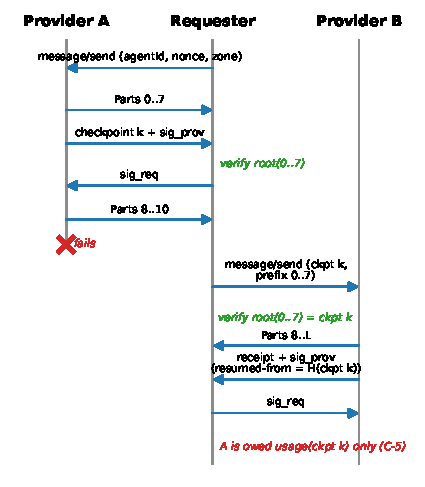
\includegraphics[width=\columnwidth]{figs/flow}
  \caption{A \sys{} task over A2A. Provider~A proposes checkpoints and the
  requester countersigns each one after recomputing the transcript root.
  When A fails, the requester resumes on Provider~B from the last
  countersigned checkpoint. B verifies the replayed prefix before it
  continues. B's work ends in a dual-signed receipt that names the
  checkpoint it resumed from. A is owed only the usage in that checkpoint
  (C-5).}
  \label{fig:flow}
\end{figure}

\subsection{Identity and encoding}
An agent is an Ed25519~\cite{rfc8032} public key (its AgentID). Every
artifact is a map in deterministic CBOR~\cite{rfc8949}. Each signature
covers a role-tagged signing input, $\mathit{enc}([\mathit{tag},
\mathit{role}, \mathit{core}])$, where the tag is \eg\texttt{"MAPReceipt"},
and the signature is carried either detached or in COSE\_Sign1~\cite{rfc9052}.
One invariant runs through all verification: a verifier checks signatures
over the bytes it \emph{received}, never over a re-serialization of
decoded values. That rules out a class of malleability bugs in which two
encodings of ``the same'' object verify differently. \sys{} fixes one
algorithm suite (Ed25519 and SHA-256) and negotiates nothing.

\subsection{Dual-signed execution receipts}
\label{sec:receipts}
A receipt's signed core names the task, the requester, the provider, the
capability, the start and end times, the outcome and the cumulative usage.
It optionally adds a rating, a voucher digest, the transcript root, the
data-sensitivity zone, and the checkpoint the task resumed from. Over A2A,
the provider proposes the receipt when the task reaches a terminal state,
and the requester countersigns it. The requester countersigns only if the
usage is within its own tolerance of what it observed; the tolerance is
local policy.

A receipt is \emph{admissible} evidence only if it passes four rules:
\begin{description}
\item[R-1] Each present signature verifies over the received bytes, and
  its signer is exactly the party named in the core.
\item[R-2] The requester and provider differ.
\item[R-3] \texttt{started} $\le$ \texttt{ended}, and \texttt{ended} is
  not in the evaluator's future beyond a skew bound (default 120\,s).
\item[R-4] Only a receipt signed by \emph{both} parties can be positive
  evidence. A requester-only receipt can only be negative (failed,
  timed out or disputed). A provider-only receipt counts for nothing.
\end{description}
R-4 is what makes evidence \emph{mutual}. A provider cannot mint praise
for itself, and a requester's complaint is attributable to that requester.
A provider that refuses to countersign its own failures (``selective
countersigning'') cannot suppress them, because the requester files a
unilateral negative receipt instead.

R-4 does \emph{not} stop a Sybil ring. The attacker there holds both
keys, so every receipt is genuinely dual-signed. Issuer weighting
(\S\ref{sec:trust}) is what closes it.

\subsection{Observer-local trust}
\label{sec:trust}
\paragraph{Rebuild rule.}
Trust is a \emph{projection}: derived data that any observer can
recompute from its receipt store. The rules:
\begin{itemize}
\item \textbf{T-1.} Rebuilding from the store must reproduce any
  incrementally maintained projection exactly. Decay uses the receipt's
  \texttt{ended} time, never the ingestion time, so arrival order does not
  matter.
\item \textbf{T-2.} R-1 to R-4 are part of the projection's
  \emph{apply} step, shared by incremental ingestion and by rebuild.
  Neither path can skip them.
\end{itemize}
We found T-2 the hard way. The first implementation checked the
dual-signature gate only on ingestion, so a rebuild silently admitted
unilateral positive receipts. An earlier review exploited exactly that
gap. It ran as AI-model sessions with no access to the implementation work
(Acknowledgments).

\paragraph{Scoring.}
The recommended score is Beta reputation~\cite{josang2002beta}. For each
admissible receipt $r$ about subject $s$ and capability $c$, let
$w(r) = \mathit{iw}(r)\cdot\lambda^{\Delta t}$, with decay
$\lambda = 0.98$ per day. Positive outcomes add $w(r)$ to $\alpha_{sc}$,
and failures add it to $\beta_{sc}$. The score is
$\alpha/(\alpha+\beta)$ under a $(1,1)$ prior. Its confidence
$\alpha+\beta$ is reported separately, because a score of 1.0 from one
receipt and a score of 0.97 from five hundred are different claims.
One issuer's total contribution to a subject is capped at 50 units, after
weighting.

\paragraph{Issuer weighting.}
\textbf{T-3} fixes the endpoints of the issuer weight $\mathit{iw}$: the
observer's own receipts weigh 1, and an issuer with no evidence
relationship to the observer weighs \emph{zero}. Zero, and not the
Beta prior's neutral 0.5, is the fix for receipt farming. In the ablation
where unknown issuers weigh 0.5, attackers win 72\% of honest requesters'
tasks under farming at $\alpha{=}0.2$, versus 2.5\% with weight 0
(\S\ref{sec:eval-trust}).

Between the endpoints, \sys{} compares three weightings:
\begin{itemize}
\item \textbf{W0} (self only) uses nothing but the observer's own
  receipts.
\item \textbf{W1} (direct agreement) weighs issuer $i$ by
  $a(o,i)=\max(0,\,1-2\cdot\mathrm{MAD}(o,i))$. The MAD is the mean
  absolute difference between $i$'s and the observer's per-provider
  success rates, taken over providers that both have rated at least 3
  times. At least 3 shared providers are required, or the weight is 0.
  This is the similarity weighting of PeerTrust and
  Credence~\cite{xiong2004peertrust,walsh2006credence}.
\item \textbf{W2} (propagation) is personalized
  PageRank~\cite{page1999pagerank}, in the spirit of
  EigenTrust~\cite{kamvar2003eigentrust}, over the row-normalized
  agreement graph of all issuers: 10 steps with restart 0.15 to the
  observer, and $\mathit{iw}(i)=\min(1,t_i/t_o)$.
\end{itemize}
The specification recommends \textbf{W1}. \S\ref{sec:eval-trust} explains
why this differs from our pre-registered choice.

\subsection{Countersigned checkpoints and resumption}
\label{sec:checkpoints}
\paragraph{Transcript.}
The provider's output Parts form a Merkle tree over SHA-256. A leaf is
$H(\mathtt{0x00}\,\|\,\mathit{enc}([\mathit{seq},\mathit{kind},
\mathit{content}]))$ and an interior node is
$H(\mathtt{0x01}\,\|\,l\,\|\,r)$. The domain separation rules out
leaf/interior confusion.

\paragraph{Checkpoints.}
A \texttt{CheckpointArtifact} signs a core with these fields:
\begin{itemize}
\item the task, requester and provider;
\item \texttt{through-seq};
\item the transcript root over Parts $0..\mathit{through\text{-}seq}$;
\item cumulative usage and the zone;
\item optionally, a voucher digest and a resumed-from digest.
\end{itemize}
The signing order is fixed:
\begin{itemize}
\item \textbf{C-1.} The provider signs first.
\item \textbf{C-2.} The requester countersigns only after recomputing the
  root from the Parts it actually received.
\item \textbf{C-3/C-4.} \texttt{through-seq} strictly increases between
  checkpoints, and usage never decreases.
\end{itemize}
A checkpoint with both signatures is a \emph{valid resumption point}.

\paragraph{Resumption.}
When a provider fails, the requester sends a successor the last valid
resumption point together with the transcript prefix it covers. The
successor recomputes the root and refuses to continue on any mismatch.
Its own receipt carries \texttt{resumed-from}, the digest of that
checkpoint. The providers need not know each other, and continuation need
not be deterministic across them: the seam is visible in the transcript.

\paragraph{Scope of resumption.}
The transcript holds only the Parts a provider delivered. Resuming from
it is complete only for tasks whose state \emph{is} their output, such as
streamed generation. A provider's hidden state is not in the transcript,
including tool results, scratchpads and working files. A successor also
cannot see external side effects its predecessor caused, such as a
payment or a write, so it may repeat them. \sys{} does not make such
effects idempotent. Tasks that have them need application-level
checkpoints or idempotency keys, which are outside this layer.

\paragraph{Billing bound.}
\textbf{C-5}: a failed provider is owed only the usage in its last
countersigned checkpoint. It is never owed a figure it claimed
afterwards. Overbilling is therefore bounded by one checkpoint interval
$c$. The default (C-6) depends on how countersignatures travel. It is
$c{=}8$ Parts when they return asynchronously while the task keeps
running, and $c{=}32$ when the provider pauses for each one. Both come
from the evaluation (\S\ref{sec:eval-checkpoint},
\S\ref{sec:eval-meter}).

\subsection{Evidence-bound metering}
\label{sec:metering}
\sys{} does not move money. Checkpoints and receipts may carry
\texttt{voucher-digest}, the hash of the payer-signed cumulative voucher
that covers the usage they record. This is a \emph{reverse} binding.
The rail's voucher format is untouched, yet anyone holding both artifacts
can prove they refer to the same delivery. A requester should not sign a
voucher beyond the price of its last countersigned checkpoint plus the
credit it deliberately extends (M-6). Pausing and resuming delivery are
left to the rail: MPP's session updates and x402's batch
settlement~\cite{mpp2026,x402v2}. Amounts are unsigned integers. A
negative amount therefore cannot be encoded, which removes a v1 bug in
which a negative payment moved funds backwards.

\subsection{Zones}
\label{sec:zones}
A task carries a data-sensitivity label $z\in\{0..3\}$, from local-only
to open. A counterparty's zone is the \emph{requester's} classification
of it (allowlisted, authenticated mesh peer, or ephemeral), never the
provider's own claim.
\begin{itemize}
\item \textbf{Z-1.} A zone-$z$ task may go only to a counterparty
  classified $\le z$.
\item \textbf{Z-2.} The label is inside the dual-signed checkpoint and
  receipt, so a provider cannot later deny the handling obligation it
  accepted.
\item \textbf{Z-3.} A label never widens along a resumption chain.
\end{itemize}
Zones make mishandling attributable, not impossible.

\subsection{Two-plane discovery}
\label{sec:discovery}
The \emph{stable plane} holds signed descriptors, which embed the
provider's signed A2A Agent Card (\S\ref{sec:binding}). They are
published into a Kademlia DHT under sharded capability keys
$K(\mathit{cap},s)$, with $s=\mathrm{SHA\text{-}256}(\mathit{AgentID})[0]$.
A querier samples a few random shards and merges the results. The DHT is
untrusted storage.
\begin{itemize}
\item \textbf{D-6.} The querier discards any record whose AgentID does not
  belong in the shard it was found under, and verifies every descriptor
  signature before shortlisting it.
\item \textbf{D-9.} Queriers should use $d{=}3$ disjoint-path lookups, in
  the style of S/Kademlia~\cite{baumgart2007skademlia}.
\end{itemize}
The \emph{volatile plane} (queue length, estimated latency) is pulled on
demand from the shortlist with a \texttt{StatusQuery}. It is not
carried in descriptors, because a cached value is stale when it matters
(\S\ref{sec:eval-discovery}).

\section{Binding to A2A}
\label{sec:binding}

\sys{} is an A2A~v1.0 extension. Its URI appears in the Agent Card under
\texttt{capabilities.extensions}, with \texttt{required} left false. A
client activates the extension per request with the
\texttt{A2A-Extensions} header. A provider that does not recognize the
extension, or a client that does not ask for it, gets a plain A2A
interaction (G5).

\paragraph{Where artifacts ride.}
Each \sys{} artifact travels as base64url of its CBOR bytes, under one
namespaced key, \texttt{"map/v2"}, in A2A \texttt{metadata}:
\begin{itemize}
\item \textbf{Opening message:} carries the requester's AgentID, a
  16-byte task nonce and the zone label.
\item \textbf{Checkpoint proposals:} ride on a status-update event that
  leaves the task \textsc{working}. The countersignature comes back
  asynchronously in a message to the running task.
\item \textbf{Fallback:} A2A leaves it to the implementation whether a
  client can send a message mid-\textsc{working}. A provider therefore
  must also support pausing in a transient \textsc{input-required} state
  to collect the countersignature.
\item \textbf{Receipt:} the provider proposes it at the terminal state.
\end{itemize}

\paragraph{TaskID and transcript leaves.}
The A2A task identifier is chosen by the provider, so it cannot name the
task on its own. \sys{} derives
\[
\mathit{TaskID} = \mathrm{SHA\text{-}256}(\mathit{enc}([
\texttt{"MAPTaskID"}, \mathit{nonce}, \mathit{provider}, \mathit{a2aTaskId}])).
\]
This binds the requester's freshness, the provider's identity and A2A's
handle together. The transcript leaves are the Parts the provider
delivers. A leaf's content is the RFC~8785 (JCS)~\cite{rfc8785} canonical
JSON of the Part, so two implementations that parse and re-serialize a
Part still agree on the root.

\paragraph{Resumption.}
Resuming is an ordinary new A2A task at the successor. Its opening
message lists the failed task in \texttt{referenceTaskIds}. It carries the
countersigned checkpoint in metadata, and carries the transcript prefix as
a \texttt{DataPart}.

\paragraph{Descriptors embed the Agent Card.}
A \sys{} descriptor is a COSE-signed map containing:
\begin{itemize}
\item the Agent Card's JCS bytes and its JWS signature;
\item the capability keys, a sequence number and a TTL;
\item the accepted zones.
\end{itemize}
The JWS key must be the AgentID key. Discovery results are therefore
self-verifying A2A Agent Cards, and an agent needs one identity, not two.

\section{Implementation}
\label{sec:implementation}

\paragraph{Rust.}
The reference implementation is 8,040 lines of Rust across ten crates:
identity, core encoding and envelopes, transcript and checkpoints, trust,
metering, discovery, the libp2p discovery node, and supporting crates.
It also includes a 2,535-line A2A adapter (provider middleware, requester
client, card and descriptor signing) and a 976-line conformance suite.
The trust crate's \texttt{apply} function enforces R-1 to R-4 for both
incremental ingestion and rebuild (T-2). Tests check that the two paths
agree, including on mixed streams of forged, unilateral and dual-signed
receipts. The workspace has 167 tests.

\paragraph{Go.}
A second, full implementation (9,274 lines, standard library only) covers
the same layers, including an A2A provider and requester. It is
\emph{not} independent in the IETF sense: the same author and model
family produced it with the Rust source available. It does give a second parser and signer for
every artifact, and it found real ambiguities in the specification. It
has 78 top-level tests.

\paragraph{Interoperability.}
\begin{itemize}
\item \textbf{Vectors.} Seventeen live test vectors pin every artifact
  byte for byte: receipts, checkpoints, descriptors, signed Agent Cards,
  admissibility decisions, TaskIDs and transcript leaves. Both
  implementations reproduce all of them.
\item \textbf{Live matrix.} A 28-cell matrix runs every combination of
  Rust and Go as requester, provider~A and provider~B through a
  kill-and-resume task over A2A HTTP. It also runs plain A2A clients
  against \sys{} providers, and the core session cells. All 28 pass.
\item \textbf{Unmodified SDK.} The official A2A Python SDK
  (a2a-sdk~1.0.3), unmodified, does the following against our provider:
  \begin{itemize}
  \item resolves its Agent Card;
  \item verifies the card's signature with the SDK's own verifier;
  \item rejects the card once one field is altered (a negative control);
  \item completes a plain task.
  \end{itemize}
\end{itemize}

\paragraph{A canonicalization pitfall.}
Our first signed Agent Card verified under our reading of the A2A
specification but failed the Python SDK's EdDSA verifier. The SDK
canonicalizes a card by converting it with protobuf's
\texttt{MessageToDict}, dropping every empty value, and serializing with
sorted keys. That differs from the specification's rule, which applies
RFC~8785 after removing only non-required empties. The difference shows
up in exactly the constructs we had used:
\begin{itemize}
\item \texttt{"required": false}, a proto3 implicit-presence default;
\item integers inside a \texttt{google.protobuf.Struct}, which protobuf
  re-serializes as doubles (\texttt{32.0}).
\end{itemize}
The binding now includes an interop profile: no empties, no implicit
defaults, no JSON numbers in \texttt{Struct}s, and ASCII only. Cards
within that profile produce identical bytes under both rules. We report
this because every signed-Agent-Card deployment faces the same trap.

\paragraph{Simulator.}
\texttt{map-sim} (3,057 lines) is a deterministic discrete-event
simulator.
\begin{itemize}
\item \textbf{Real crates.} It calls the real crates for admissibility,
  transcripts, checkpoints, metering and shard checks. Only signing can
  be replaced, by a fast mode; a fixed-seed test shows the fast mode
  produces byte-identical output.
\item \textbf{Randomness.} Every run draws from ChaCha8, seeded by
  SHA-256 of (scenario, point, seed).
\item \textbf{Reproducible output.} Results are written in job order, so
  the output CSV is byte-identical at any thread count.
\item \textbf{Weighting check.} A test compares the fast W1 and W2
  implementations with their direct definitions for exact equality. We
  validated it by planting a bug and checking that it fails.
\end{itemize}
Criterion benchmarks on one core of a Ryzen~7 5800X measure:
\begin{itemize}
\item a dual-signed receipt (encode, two signatures, two verifications):
  $127\,\mu$s;
\item a checkpoint cycle (propose, countersign, verify): $126\,\mu$s;
\item appending a Part and recomputing the transcript root:
  $1.3\,\mu$s.
\end{itemize}
A receipt is 327 bytes, and a checkpoint 312.

\section{Evaluation}
\label{sec:evaluation}

\subsection{Method}
\label{sec:eval-method}

\paragraph{Pre-registration.}
We committed and tagged every hypothesis, decision rule and predicted
losing regime (\texttt{prereg-v1}) \emph{before} writing the simulator.
We did this because one author, working with a single AI model family
(Acknowledgments), produced \sys{}, the baselines and the simulator.
That is the main threat to validity~\cite{nosek2018prereg}.
After the tag, the plan changed only through dated, appended amendments
(A1--A11, Appendix~\ref{app:amendments}), and we report every hypothesis
whatever its outcome. Two amendments changed a decision and are disclosed
where they apply:
\begin{itemize}
\item \textbf{A4} repaired the weighting decision rule after we had seen
  plumbing-test numbers (\S\ref{sec:eval-trust}).
\item \textbf{A9}, requested by the author after an exploratory finding,
  re-chose the recommended weighting with a new rule. That rule was
  committed and pushed before its run.
\end{itemize}

\paragraph{Statistics.}
Each sweep point runs 20 seeds (60 for F1, matching its source). We report
means with 95\% percentile-bootstrap CIs over seeds (10,000
resamples~\cite{efron1993bootstrap}). A comparative hypothesis
\emph{holds at a point} only if the CI of the difference or ratio lies
entirely on the claimed side. Seeds are resampled jointly for paired
arms. We apply no multiple-comparison correction, and the full grid is
published.

\paragraph{Reproducibility.}
One command (\texttt{eval/run\_all.ps1}) builds the simulator, checks the
golden hashes, runs every experiment, and regenerates the report and the
figures. We ran the whole evaluation twice, at two commits:
\begin{itemize}
\item \textbf{Byte-identical outputs.} Every experiment that ran in both
  runs produced byte-identical CSVs.
\item \textbf{Run once.} The main trust grid ran only at the second
  commit, after a cache-blocking optimization verified to be bit-identical
  (A7). The two follow-up weighting sweeps (A8, A9) also ran once.
\item \textbf{Signing modes.} Real and fast signing produce identical
  output on a check grid, re-verified on every run (A1).
\end{itemize}

\begin{table}[t]
\caption{Pre-registered verdicts (20 seeds; F1: 60). ``Holds'' counts the
points whose 95\% CI lies on the claimed side. L1--L4 are
\emph{predicted} losing regimes, so ``occurs'' is a loss for \sys{}.}
\label{tab:verdicts}
\small
\begin{tabular}{@{}llr@{}}
\toprule
Id & Claim & Verdict \\
\midrule
F1-a & Replicates~\cite{wang2026agenticp2p} Fig.~5a within $\pm$0.05 & holds 12/12 \\
F1-b1 & At 60\,s, \sys{} adds nothing to Risk-Aware & partial 5/6 \\
F1-b2 & At 3600\,s, \sys{}+RA $-$ RA $\ge 0.10$ & holds 4/4 \\
F1-b3 & \ldots\ under 60\,s whitewashing, $\ge 0.05$ & holds 2/2 \\
H1 & Attacker share $\le 0.5\times$ B1 and B2 & \textbf{partial 18/28} \\
L1 & Cold start: worse than B2, rounds 1--5 & occurs 35/35 \\
L2 & Sparse evidence: W0 $\not<$ random & did not occur \\
L3 & On-off: decay lags the off phase & occurs 5/5 \\
L4 & Camouflage hurts W1/W2 ($\alpha{=}0.2$) & did not occur \\
H2 & Resume waste $\le 0.4\times$ restart & holds \\
H3 & D-6 caps flooding at fair share & holds 6/6 \\
H4 & Pulled status beats descriptor-carried & holds 4/4 \\
H5 & Exposure $\le$ price($c$); CPU overhead $<$1\% & holds 6/6 \\
\bottomrule
\end{tabular}
\end{table}

\subsection{Replicating an agentic P2P baseline}
\label{sec:eval-f1}
Before comparing against Wang et al.'s Risk-Aware
policy~\cite{wang2026agenticp2p}, we re-implemented their simulator's model
from its source code. We read that code but did not execute it. The model:
\begin{itemize}
\item 100 peers, a fraction $\alpha$ of them Sybils that overclaim their
  self-reported hints and succeed 5\% of the time;
\item two-step workflows, a shortlist of 25, and up to three attempts
  per step;
\item a canary that honest peers pass 97\% of the time and Sybils 8\%.
\end{itemize}
Our curves match their published Fig.~5a at all 12 points to within
$\pm$0.05; the largest difference is 0.024 (Figure~\ref{fig:f1}). This
gate had to pass before any comparison.

We then added \sys{}'s local projection, evaluated in their world:
\begin{itemize}
\item \textbf{Short horizon.} In their 60\,s horizon, a requester has
  less than one workflow of its own history. As predicted, \sys{}
  ranking in front of the canary (\sys{}+RA) adds nothing at five of six
  values of $\alpha$. The exception is $\alpha{=}0.3$, a small gain of
  $+0.037$\ci{0.002}{0.071}.
\item \textbf{One hour.} At 3,600\,s, evidence accumulates and \sys{}+RA
  beats Risk-Aware by 0.123 to 0.265 for $\alpha\in[0.2,0.5]$.
\item \textbf{Whitewashing.} With Sybils re-keying every 60\,s, it still
  beats Risk-Aware by 0.105 at $\alpha{=}0.2$ and 0.169 at
  $\alpha{=}0.3$, because honest providers keep their history.
\end{itemize}
Risk-Aware verifies each task; it does not remember the result. \sys{}
supplies the memory.

\begin{figure}[t]
  \centering
  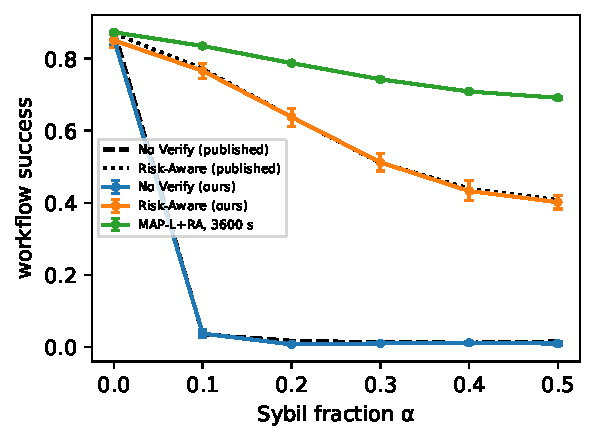
\includegraphics[width=0.9\columnwidth]{figs/f1_replication}
  \caption{Replication of~\cite{wang2026agenticp2p} Fig.~5a (dashed:
  published; solid: ours, 60 seeds, 95\% CIs) and \sys{}'s local
  projection with the canary over a 3,600\,s horizon.}
  \label{fig:f1}
\end{figure}

\subsection{Trust under attack (E1)}
\label{sec:eval-trust}

\paragraph{World.}
The simulated world has:
\begin{itemize}
\item 200 providers and 500 honest requesters over 60 rounds; one round
  is one day of decay;
\item Poisson(2) tasks per requester per round;
\item a shortlist of 10 providers per task, with 10\% uniform
  exploration and up to 3 attempts.
\end{itemize}
Honest providers succeed with $q\sim U[0.80,0.98]$. A fraction $\alpha$
of providers is adversarial, with $q{=}0.2$. Adversarial providers refuse
to countersign their failures. In the Sybil attacks (farming, camouflage,
slander, combined), each one also controls 20 Sybil requesters.
Every receipt goes to one public pool, the worst case. Discovery is
honest: shortlists are drawn from the real providers only
(\S\ref{sec:eval-discovery} drops this assumption). The metric is the
steady-state (rounds 31--60) share of honest requesters' tasks that go to
adversarial providers.

\paragraph{Arms.}
\begin{itemize}
\item \textbf{B0}: random selection.
\item \textbf{B1}: a global ledger in the style of ERC-8004. It is
  \sys{}'s own projection with every issuer weighted~1; it keeps the
  decay and the cap, which makes it a \emph{stronger} baseline than a raw
  sum (A3).
\item \textbf{B2}: Risk-Aware's canary.
\item \textbf{B2L}: B2 plus a ledger of provider-signed receipts, the
  paper's prose design.
\item \textbf{Ours-L}: \sys{}.
\item \textbf{Ours-L+C}: \sys{} with the canary in front.
\item \textbf{Ablations:} unknown issuers weighted 0.5
  (\emph{A-prior}); requester-only positive receipts admitted
  (\emph{A-unilateral}).
\end{itemize}

\begin{figure*}[t]
  \centering
  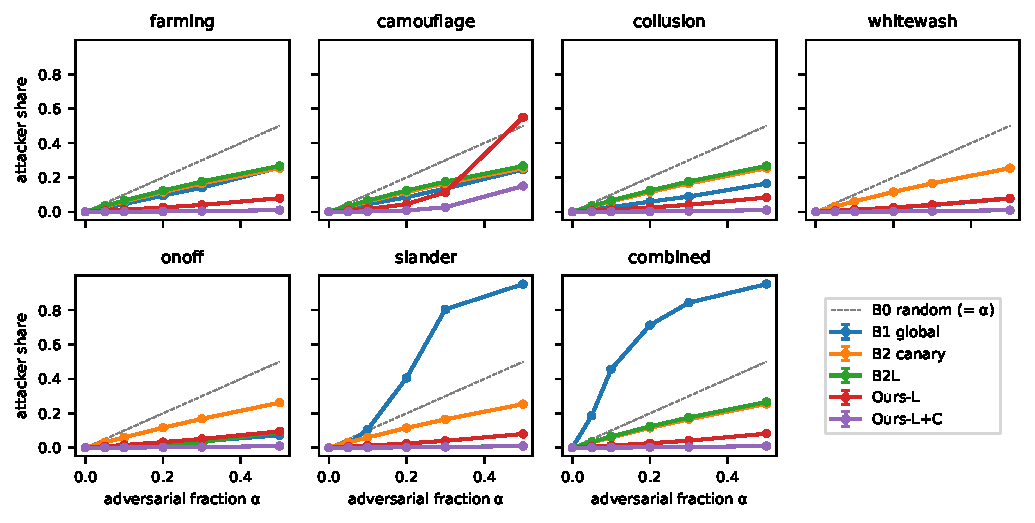
\includegraphics[width=\textwidth]{figs/e1_attacker_share}
  \caption{E1: steady-state attacker share of honest requesters' tasks
  versus adversarial fraction $\alpha$ (20 seeds, 95\% CIs). The dashed
  line is random selection. Ours-L uses the pre-registered weighting, W2;
  Table~\ref{tab:w1h1} gives the recommended W1.}
  \label{fig:e1}
\end{figure*}

\paragraph{Results (Figure~\ref{fig:e1}).}
H1 is only \textbf{partially} supported: Ours-L's attacker share is at
most half of both baselines' at 18 of 28 points. Against the canary
baseline B2 it holds at 27 of 28 points. The exception is camouflage at
$\alpha{=}0.3$, with a ratio of 0.69. Against the global ledger B1, H1
fails in three families:
\begin{itemize}
\item \textbf{Whitewashing.} The ratio is about 1.04 at every $\alpha$.
  Fresh identities have no evidence under \emph{either} scheme, so both
  sit at the floor set by exploration and fallback. Halving that floor
  is not possible.
\item \textbf{On-off.} The ratio is about 1.4. B1 pools every issuer's
  evidence, so it sees the ``off'' phase sooner than an observer that
  trusts only issuers resembling itself.
\item \textbf{Camouflage at $\alpha\ge0.2$.} Discussed below.
\end{itemize}
In the other direction, the global ledger \emph{collapses} under slander:
\begin{itemize}
\item B1's attacker share is 0.406 at $\alpha{=}0.2$ and 0.952 at
  $\alpha{=}0.5$. Sybil complaints bury honest providers, and the
  adversaries inherit the traffic.
\item Ours-L stays at 0.025 and 0.080, because complaints from issuers
  that disagree with the observer weigh nothing.
\item Under combined attacks B1 reaches 0.713 at $\alpha{=}0.2$.
\end{itemize}
\paragraph{Ablations.}
A-prior confirms T-3. With unknown issuers weighted 0.5 (the v1 design),
farming wins 0.715 of tasks at $\alpha{=}0.2$; with weight 0 it wins
0.025.

A-unilateral does \emph{not} test R-4, and we do not claim it does. In
E1 no agent emits a receipt that R-4 would stop from counting as
positive evidence:
\begin{itemize}
\item honest successes are dual-signed;
\item farming is dual-signed too, because the attacker holds both keys;
\item the only single-signed receipts are negative ones.
\end{itemize}
The arm therefore admits a receipt type that never occurs, and its
attacker share differs from Ours-L's by at most 0.0023 in any cell. That
difference is noise between independent random streams. What E1 measures
is issuer weighting (T-3). R-4's protection against a lone provider
minting its own praise (G1) is argued in \S\ref{sec:security}, not
measured.

\paragraph{The canary and Wang et al.'s full design.}
The canary composes with \sys{}: Ours-L+C keeps the attacker share at or
below 0.15 in every cell, and at or below 0.004 in every cell with
$\alpha\le0.3$ except camouflage.

B2L, the canary plus a provider-signed ledger, is the design Wang et al.'s
prose describes, and Figure~\ref{fig:e1} plots it. H1 did not
pre-register a comparison with it, so the one below is exploratory
(Table~\ref{tab:b2l}). The arms do not share random streams, so each is
resampled independently.
\begin{itemize}
\item \textbf{Ours-L+C against B2L.} Across all 35 cells, Ours-L+C is
  lower in 25 and never higher. It is lower in every cell under farming,
  camouflage, collusion, on-off and combined attacks, and the CIs overlap
  in the other ten (whitewashing and slander).
\item \textbf{Ours-L alone against B2L.} Without a canary, Ours-L is
  higher than B2L under whitewashing and slander at every $\alpha$, and
  under on-off at four of five. B2L's canary catches fresh identities,
  and its ledger admits only provider-signed receipts, so Sybil
  complaints never reach it.
\item \textbf{Where B2L is weak.} B2L's ledger is open to farming: at
  $\alpha{=}0.2$ it gives adversaries 0.123 of tasks, against 0.025 for
  Ours-L and 0.002 for Ours-L+C.
\end{itemize}

\begin{table}[t]
\caption{Exploratory: B2L (canary + provider-signed ledger) against
\sys{}, steady-state attacker share at $\alpha{=}0.2$, W2 weighting
(20 seeds; every 95\% CI is within $\pm$0.004 of the mean). All 35 cells
are in \texttt{B2L.md}.}
\label{tab:b2l}
\small
\begin{tabular}{@{}lrrr@{}}
\toprule
Attack & B2L & Ours-L & Ours-L+C \\
\midrule
farming & 0.123 & 0.025 & 0.002 \\
camouflage & 0.124 & 0.045 & 0.008 \\
collusion & 0.124 & 0.025 & 0.002 \\
whitewash & 0.002 & 0.025 & 0.002 \\
on-off & 0.018 & 0.033 & 0.002 \\
slander & 0.002 & 0.025 & 0.002 \\
combined & 0.124 & 0.026 & 0.002 \\
\bottomrule
\end{tabular}
\end{table}

\paragraph{Losing regimes.}
All four predicted losing regimes were tested:
\begin{itemize}
\item \textbf{Cold start (L1): occurs everywhere.} In rounds 1--5,
  Ours-L without the canary has a higher attacker share than B2: by
  0.014 at $\alpha{=}0.05$, up to 0.217 at $\alpha{=}0.5$. Local trust
  needs history, and a deployment should run a canary until it has some.
\item \textbf{On-off (L3): occurs.} At the start of each off phase the
  attacker share exceeds steady state by 0.017 to 0.196, the lag of a
  0.98/day decay.
\item \textbf{Sparse evidence (L2): did not occur.} At 0.1 tasks per
  requester per round, self-only weighting still beat random, by 0.9 to
  2.3 points.
\item \textbf{Camouflage (L4): did not occur at the pre-registered
  $\alpha{=}0.2$.} Agreement-based weights were not worse than self-only
  there. At higher $\alpha$ they were, as described next.
\end{itemize}

\paragraph{Detection time and whole-run share.}
Two further pre-registered E1 metrics are in \texttt{PREREG-EXTRA.md}.
\emph{Time to detect} is the first round from which the attacker share,
averaged over five rounds, is at most $\alpha/4$.
\begin{itemize}
\item \textbf{Ours-L} reaches $\alpha/4$ after 26--33 rounds with W2 and
  27--38 with W1 in 34 of 35 cells. It never does under camouflage at
  $\alpha{=}0.5$.
\item \textbf{The canary alone (B2)} never reaches it in any cell: it
  holds the attacker to $0.51$--$0.62\alpha$.
\item \textbf{B1} never reaches it in 18 of 35 cells, and \textbf{B2L}
  in 20.
\item \textbf{Ours-L+C} is below it from the first round in every cell.
\end{itemize}
Over all 60 rounds, which include the cold start, Ours-L's attacker share
is about three times its steady-state value (0.076 against 0.025 at
$\alpha{=}0.2$ under farming). Ours-L+C stays at or below 0.023 for
$\alpha\le0.3$ and reaches at most 0.098 at $\alpha{=}0.5$.

\paragraph{Choosing the weighting: a pre-registered rule, a collapse,
and a re-test.}
The pre-registered rule compared W0/W1/W2 at $\alpha{=}0.2$ only.
Averaged over all attacks, the steady-state attacker shares were:
\begin{itemize}
\item W0: 0.0796;
\item W1: 0.0312;
\item W2: 0.0290.
\end{itemize}
It selected W2 (A6). One disclosure applies: the rule's tie clause, as
first written, was satisfied almost always, and it would have chosen W0.
We repaired it (A4) \emph{after} seeing two-seed plumbing numbers, and
report both readings.

The main grid then showed W2 \emph{worse than random} under camouflage
at $\alpha{=}0.5$: 0.550, against 0.500 for random selection. At that
point 2,000 camouflaging Sybils face 500 honest requesters. Their
truthful reports about honest providers earn them agreement edges, and
propagation concentrates the observer's trust mass in the Sybil cluster.
This is the classic weakness of transitive trust against Sybils who have
bought honest-looking edges~\cite{yu2006sybilguard,cheng2005sybilproof}.
We had not tested it at that $\alpha$.

An exploratory run confirmed the collapse and showed that W1 does not
suffer it (A8). We then pre-registered a minimax rule (A9) and pushed it
before its run: choose the weighting with the lowest worst-case attacker
share over all 35 ($\alpha$, attack) cells. Table~\ref{tab:minimax}
gives the worst cells; Figure~\ref{fig:minimax} shows the two families
where the weightings differ most.

W1 wins, with non-overlapping CIs, and the specification recommends it.
The price is small. Outside on-off and camouflage, W2 is ahead by at most
0.003 at $\alpha\le0.3$ and by at most 0.007 at $\alpha{=}0.5$. Under
on-off it is ahead by 0.003 to 0.040. H1 and the other E1
verdicts stay as pre-registered, computed with W2.

\paragraph{H1 for the recommended weighting (exploratory).}
Every E1 headline above uses W2, which the specification no longer
recommends. Table~\ref{tab:w1h1} applies the H1 criterion to W1 instead.
W1's cells come from a separate run with independent random streams, so
each ratio's CI resamples the two arms independently. W2 is recomputed
the same way. That reproduces its pre-registered counts exactly: 18 of
28 points, and 27 of 28 against B2 alone.
\begin{itemize}
\item \textbf{Overall.} With W1, H1 holds at 17 of 28 points, and
  against the canary alone at all 28.
\item \textbf{Where W1 differs from W2.} It passes camouflage against B2
  at $\alpha{=}0.3$, with a ratio of 0.44 where W2 had 0.69. It fails
  collusion at $\alpha{=}0.3$, with a ratio of 0.49 whose upper bound is
  0.51. Both calls turn on margins of about 0.01.
\item \textbf{Against the global ledger under on-off} W1 is further
  behind than W2: a ratio of 1.85--1.94, against about 1.4.
\item \textbf{The slander result holds for W1:} 0.027 at $\alpha{=}0.2$
  and 0.084 at $\alpha{=}0.5$, against B1's 0.406 and 0.952.
\end{itemize}

\begin{table}[t]
\caption{Exploratory: the H1 criterion (Ours-L at most half of both B1
and B2, upper CI $\le$ 0.5) for W2 and W1, per attack, over the
pre-registered $\alpha\in\{0.05,0.1,0.2,0.3\}$. The arms are resampled
independently. The ratio columns give W1's range of point estimates over
$\alpha$. All cells are in \texttt{W1-H1.md}.}
\label{tab:w1h1}
\small
\begin{tabular}{@{}lrrrr@{}}
\toprule
Attack & W2 holds & W1 holds & W1/B1 & W1/B2 \\
\midrule
farming & 4/4 & 4/4 & 0.28--0.31 & 0.20--0.26 \\
camouflage & 2/4 & 2/4 & 0.40--0.53 & 0.28--0.44 \\
collusion & 4/4 & 3/4 & 0.45--0.49 & 0.20--0.26 \\
whitewash & 0/4 & 0/4 & 1.05--1.08 & 0.19--0.25 \\
on-off & 0/4 & 0/4 & 1.85--1.94 & 0.34--0.41 \\
slander & 4/4 & 4/4 & 0.05--0.24 & 0.20--0.26 \\
combined & 4/4 & 4/4 & 0.03--0.05 & 0.19--0.26 \\
\midrule
total & 18/28 & 17/28 & & \\
\bottomrule
\end{tabular}
\end{table}

\paragraph{Sybil count (exploratory, A10).}
E1 fixes 20 Sybil requesters per adversarial provider. Identities are
free, though, and W1 weights each camouflaging Sybil by its own agreement
with the observer, so nothing bounds how many count. Amendment A10,
pushed before its run, sweeps that number at $\alpha{=}0.2$
(Table~\ref{tab:sybils}):
\begin{itemize}
\item W1 held at 5 and 20 Sybils per provider, which is 0.4 and 1.6 per
  honest requester.
\item At 80, or 6.4 per honest requester, it lost to self-only weighting:
  0.077 against 0.072. At 320 it reached 0.165. It never became worse
  than random (0.2).
\item W2 was worse than random at 320 (0.526), even at $\alpha{=}0.2$.
\item Farming without camouflage stayed flat at every count, so the
  damage comes from bought agreement.
\end{itemize}
The attack is not cheap. Each camouflaging Sybil runs two real tasks per
round, so at 80 Sybils per provider the attacker buys 6.4 times the
honest workload. W1's minimax win therefore holds at the Sybil ratio of
the main grid, not in general, and the specification now says so.

\begin{table}[t]
\caption{Exploratory (A10): steady-state attacker share under camouflage
at $\alpha{=}0.2$ versus Sybils per adversarial provider (20 seeds; every
95\% CI is within $\pm$0.004 of the mean). ``Bought'' is the camouflage
tasks per round as a multiple of the honest workload. Random selection
gives 0.2.}
\label{tab:sybils}
\small
\begin{tabular}{@{}rrrrrr@{}}
\toprule
Sybils/prov. & Sybils/honest & Bought & W0 & W1 & W2 \\
\midrule
5 & 0.4 & 0.4$\times$ & 0.073 & 0.031 & 0.027 \\
20 & 1.6 & 1.6$\times$ & 0.072 & 0.041 & 0.045 \\
80 & 6.4 & 6.4$\times$ & 0.072 & 0.077 & 0.196 \\
320 & 25.6 & 25.6$\times$ & 0.072 & 0.165 & 0.526 \\
\bottomrule
\end{tabular}
\end{table}

\begin{table}[t]
\caption{A9 minimax re-test: each weighting's worst cell over
$\alpha\in\{0.05,\ldots,0.5\}\times$ seven attacks (steady-state attacker
share, 95\% CI).}
\label{tab:minimax}
\small
\begin{tabular}{@{}llll@{}}
\toprule
Weighting & Worst cell & Attacker share & Honest succ. \\
\midrule
W0 self only & 0.5, on-off & 0.348\ci{0.346}{0.350} & 0.960 \\
\textbf{W1 direct} & 0.5, camouflage & \textbf{0.200}\ci{0.196}{0.204} & 0.978 \\
W2 propagation & 0.5, camouflage & 0.550\ci{0.543}{0.557} & 0.867 \\
\bottomrule
\end{tabular}
\end{table}

\begin{figure}[t]
  \centering
  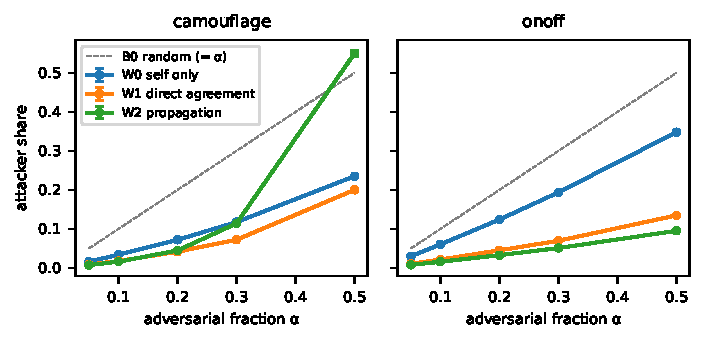
\includegraphics[width=\columnwidth]{figs/e1_minimax}
  \caption{Issuer weightings under camouflage and on-off (20 seeds, 95\%
  CIs). W2's propagation collapses once camouflaging Sybils outnumber
  honest requesters. W1 never does worse than random at the 20 Sybils per
  adversarial provider used here; Table~\ref{tab:sybils} varies that.}
  \label{fig:minimax}
\end{figure}

\subsection{Countersigned resumption (E2)}
\label{sec:eval-checkpoint}
Tasks of $L\in\{10^2,10^3,10^4\}$ Parts fail with hazard $\lambda$, with
$\lambda L\in\{0.1,1,3\}$ expected failures per task, and are resumed on
a fresh provider. We compare three recovery strategies: restarting from
scratch; resuming from a countersigned checkpoint every $c$ Parts; and
resuming from the failed provider's own claim of progress (provider-only).

\begin{itemize}
\item \textbf{H2 holds.} At $L{=}10^3$, $\lambda L{=}1$, $c{=}8$:
  \begin{itemize}
  \item countersigned resumption wastes 3.2\ci{2.8}{3.7} Parts per task;
  \item restarting wastes 768.6\ci{655.1}{881.7};
  \item the ratio is 0.0042\ci{0.0036}{0.0050}.
  \end{itemize}
\item \textbf{The billing rule (C-5) holds by construction.} The
  simulator bills a failed provider exactly its acknowledged usage.
  Its check that no run bills more than was delivered is therefore an
  invariant, not evidence. What C-5 costs is the provider's unpaid work,
  the Parts delivered after its last checkpoint. That is fewer than $c$
  per failure because the provider checkpoints every $c$ Parts. At the
  H2 operating point it averages 3.2 Parts per task. Under countersigned
  resumption, the waste above is exactly this unpaid work.
\item \textbf{Provider-only resumption} wastes nothing, whether or not
  providers are honest. With 20\% dishonest providers who overstate
  progress by 50\%, it overbills requesters by 30.2\ci{20.5}{41.3}
  Parts per task at the H2 operating point. It also causes
  0.20\ci{0.15}{0.27} transcript-integrity failures per task. At
  $\lambda L{=}3$ the figures are 53.0\ci{40.8}{66.0} and 0.45.
  Countersigned resumption has neither.
\end{itemize}

\paragraph{What H2 does and does not show.}
H2 compares countersigned resumption with restarting. Its saving belongs
to \emph{checkpointing}, not to countersigning: provider-only resumption
checkpoints too, and it wastes nothing. What countersigning buys is
safety. A dishonest provider cannot overbill, and a successor never
inherits a transcript the requester did not verify. That result follows
from the adversary model by construction, so E2 illustrates it; it does
not measure it. The measured claim is narrower: checkpointed resumption
regenerates 0.42\% of what restarting does, and countersigning adds its
safety at the cost of two signatures per checkpoint (\S\ref{sec:eval-meter}).
\paragraph{What the waste metric counts.}
E2's waste counts regenerated Parts. It does not count the successor's
cost to fetch, verify and ingest the replayed prefix. Verifying is cheap:
recomputing the root costs about $1.3\,\mu$s per Part. Ingesting is not
free. Failures arrive at rate $\lambda$ per Part of progress, and
resumption loses no progress, so the expected prefix replayed per task is
$\lambda L^2/2$. That is about 500 Parts at the H2 operating point,
against 3.2 regenerated. If ingesting a Part costs a fraction $\rho$ of
generating one, resumption costs about $3.2+500\rho$ Parts against
restart's 768.6. H2's conclusion therefore survives for any $\rho$ below
about 1.5. For language models, prefill is usually much cheaper per token
than decoding. The 0.42\% figure, however, compares regeneration only.
The specification defers an engine-state fast path that would let a
compatible successor skip ingestion. Resumption is always by transcript
replay.

Figure~\ref{fig:e2} shows the trade-off in $c$: waste grows roughly
linearly in $c$, while signatures shrink as $1/c$. Pricing a signature at
$\kappa\in\{0.01,0.1\}$ Parts of work, most settings are optimized
between $c{=}8$ and $c{=}32$. Those prices count signing only. When the
provider pauses for each countersignature, a checkpoint also costs a
round trip, and $\kappa$ rises to 1.25--2.5 per signature (\S\ref{sec:eval-meter}).
At $\kappa{=}1$ the optimum is $c{=}32$ at the H2 operating point, and
32--128 in 8 of 9 settings. The default (C-6) is therefore $c{=}8$ when
countersignatures are asynchronous and $c{=}32$ when they pause the task.

\begin{figure}[t]
  \centering
  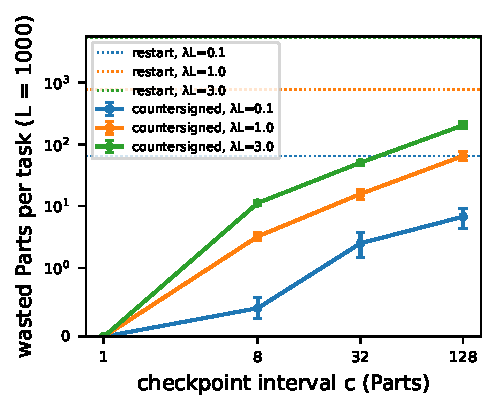
\includegraphics[width=0.85\columnwidth]{figs/e2_waste}
  \caption{E2 ($L{=}1000$): wasted Parts per task under countersigned
  resumption versus checkpoint interval $c$. Dotted lines: restart from
  scratch, in the same colour as the $\lambda L$ they match. At $c{=}1$
  no work is wasted.}
  \label{fig:e2}
\end{figure}

\subsection{Discovery (E3)}
\label{sec:eval-discovery}
\paragraph{Shard flooding (H3).}
An attacker holding a fraction $a$ of identities publishes its records
into every shard that queriers sample:
\begin{itemize}
\item \textbf{Without D-6}, it holds 46--91\% of candidates for
  $a\in\{0.01,0.05,0.1\}$.
\item \textbf{With D-6's shard check}, its share equals $a$ within 0.01
  at all six points ($n\in\{10^3,10^4\}$).
\end{itemize}

\paragraph{Identifier grinding: no mitigation.}
Generating a key pair and computing its shard costs 16.4\,$\mu$s on one
core, so an attacker makes 60,901 attempts per second.
\begin{itemize}
\item \textbf{Result.} Epoch-salted shard assignment, which re-randomizes
  every agent's shard each epoch, did not help: the attacker held
  1.000\ci{1.000}{1.000} of the target shard in all 27 configurations
  (network size, attack window, and epoch length).
\item \textbf{Why.} One core adds about 238 identities per second to any
  shard, while a shard of a $10^5$-provider network holds about 390
  honest providers. The attacker therefore has a majority about 2\,s
  after each re-salt.
\end{itemize}
A 16-core attacker, the exploratory variant of Amendment A5, also holds
the whole target shard in every configuration. When identities are free,
grinding is just targeted Sybil creation, and no shard function prevents
it. The specification now says so plainly (\S\ref{sec:security}).

\paragraph{Flooded discovery composed with trust (exploratory, A11).}
E1 assumes honest discovery, while E3b shows that discovery can be
flooded cheaply. Amendment A11, pushed before its run, composes the two.
Discovery returns $F$ zero-evidence adversarial identities alongside the
200 real providers, and every shortlist is drawn from both. It also
tests one local policy: \emph{shortlist memory}, where $k$ slots hold the
requester's best-scored providers among those it has a success receipt
for. Table~\ref{tab:flood} gives the results at $\alpha{=}0.2$ under
farming, with W1.
\begin{itemize}
\item \textbf{Without memory, trust cannot help once the flood is
  heavy.} At 10 flood identities per honest provider, discovery returns
  adversaries 91\% of the time, and Ours-L gives them 0.888 of tasks.
  Ranking cannot pick a provider that discovery never showed.
\item \textbf{Memory and the canary together protect established
  requesters.} With $k{=}3$, Ours-L+C holds the attacker to 0.036 at 10
  flood identities per honest provider and to 0.085 at 100. Honest
  success stays at 0.94 or above.
\item \textbf{New requesters are not protected.} In rounds 1--5 they have
  no memory, and Ours-L+C with $k{=}3$ still gives adversaries 0.182 and
  0.660 of tasks.
\end{itemize}
So E1's results hold only while discovery keeps returning honest
candidates. Discovery capture, not grinding into one shard, is the main
open problem.

\begin{table}[t]
\caption{Exploratory (A11): steady-state attacker share with a flooded
discovery layer ($\alpha{=}0.2$, farming, W1, 20 seeds; every 95\% CI is
within $\pm$0.008 of the mean). ``Disc.'' is the adversarial share of
discovery, which is also random selection's share. $k$ is the shortlist
memory. ``New'' is rounds 1--5.}
\label{tab:flood}
\small
\begin{tabular}{@{}rrrrrrr@{}}
\toprule
 & & \multicolumn{2}{c}{Ours-L} & \multicolumn{3}{c}{Ours-L+C} \\
Flood & Disc. & $k{=}0$ & $k{=}3$ & $k{=}0$ & $k{=}3$ & new, $k{=}3$ \\
\midrule
0 & 0.20 & 0.027 & 0.024 & 0.002 & 0.002 & 0.007 \\
1 & 0.56 & 0.211 & 0.086 & 0.023 & 0.010 & 0.032 \\
10 & 0.91 & 0.888 & 0.199 & 0.435 & 0.036 & 0.182 \\
100 & 0.99 & 0.990 & 0.634 & 0.892 & 0.085 & 0.660 \\
\bottomrule
\end{tabular}
\end{table}

\paragraph{Eclipse (E3c).}
In a simulated Kademlia (20-entry buckets, 3 parallel queries) with a
fraction $f$ of malicious routers, three disjoint lookup paths raise
lookup success at $N{=}10^5$ with $f{=}0.3$ from 0.755 to 0.930 without
churn, and from 0.906 to 0.975 with 10\% churn (Figure~\ref{fig:e3c}).
They cost 1.3--1.7$\times$ the messages. This
replicates the S/Kademlia result~\cite{baumgart2007skademlia}, and D-9
became a SHOULD.

\paragraph{Volatile plane (H4).}
Queue lengths follow an M/M/1 process. Pulling status at selection time
has lower regret than reading a value cached in a descriptor at every TTL
of 60\,s or more:
\begin{itemize}
\item at utilization 0.8 and a 600\,s TTL, the regret difference is
  $-3.40$ queue positions;
\item pulling costs 20 messages per query, against 0.02 for a
  descriptor refresh.
\end{itemize}
The pre-registered message-rate crossover favours descriptors. Pulling
costs $2K$ messages per query and refreshing costs $N/(0.8\,\mathrm{TTL})$
per second, so pulling sends fewer messages only while the query rate
$q<N/(1.6\,K\,\mathrm{TTL})$. In E3d ($N{=}K{=}10$, $q{=}1$/s) that means
any TTL above 0.63\,s. Pulling buys fresher status with messages.

\begin{figure}[t]
  \centering
  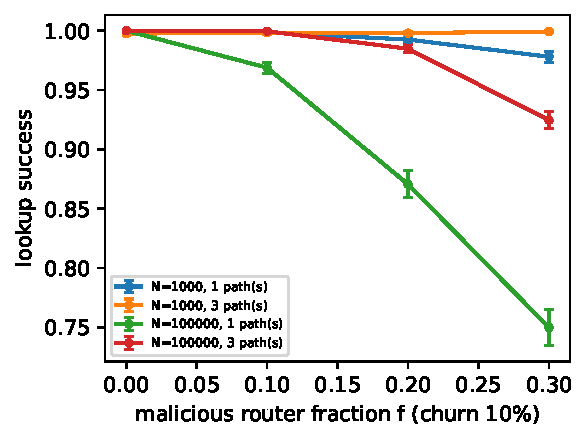
\includegraphics[width=0.85\columnwidth]{figs/e3c_lookup}
  \caption{E3c: Kademlia lookup success versus malicious-router fraction
  (10\% churn), with one path and with three disjoint paths.}
  \label{fig:e3c}
\end{figure}

\subsection{Metering (E4) and supporting evidence (E5)}
\label{sec:eval-meter}
\paragraph{Metering (H5).}
Vouchers are issued per checkpoint, with per-token prices.
\begin{itemize}
\item \textbf{Invariants.} Cumulative vouchers are monotone, re-delivery
  is idempotent, and amounts are non-negative. The simulator asserts all
  three in every run, and a provider's unpaid exposure never exceeded
  price($c$).
\item \textbf{CPU overhead.} At a generation speed of 20\,ms per token,
  \sys{} signing and verification add 0.079\% of task time at $c{=}8$,
  and 0.63\% even at $c{=}1$. This is what H5 measured, and it excludes
  the network.
\item \textbf{Round trips.} The countersignature also has to travel, and
  the cost depends on the binding's path. We estimate it rather than
  measure it, assuming a 50--100\,ms round trip.
  \begin{itemize}
  \item On the fallback path (A2A-21), the provider pauses in
    \textsc{input-required} for one round trip per checkpoint. At
    $c{=}8$, where a checkpoint covers 160\,ms of generation, that adds
    31--63\% to task time. It adds 7.8--16\% at $c{=}32$ and 2.0--3.9\%
    at $c{=}128$. Priced as work, the pause is 2.5--5 Parts per
    checkpoint.
  \item On the primary path (A2A-20), nothing pauses. Instead the
    provider keeps generating while the countersignature is in flight,
    so its unacknowledged exposure grows by 2.5--5 Parts beyond $c$.
  \end{itemize}
  Both of our implementations use only the fallback path, which every
  provider must support.
\item \textbf{Bytes.} Checkpoints are large relative to token-sized
  Parts, as the pre-registration predicted:
  \begin{itemize}
  \item at $c{=}8$ they add 38.5 bytes per Part, 4.8 times the 8-byte
    payload of a simulated Part, plus 4.25 bytes of voucher digest;
  \item at $c{=}1$ they add 308 bytes per Part, at $c{=}32$ 9.5, and at
    $c{=}128$ 2.2;
  \item these are raw CBOR sizes, and the A2A binding's base64url adds a
    third.
  \end{itemize}
  A larger $c$ is the mitigation, at the price of more waste and exposure
  (E2).
\end{itemize}

\paragraph{Formal and interop evidence (E5).}
\begin{itemize}
\item \textbf{Interop.} The interop matrix and vectors are described in
  \S\ref{sec:implementation}.
\item \textbf{Formal model.} ProVerif~\cite{proverif} proves injective
  agreement for the discovery-plane handshake's channel binding (the
  anti-relay property), with unbounded sessions. A control model that
  derives the binding without the handshake transcript fails as designed.
  Removing the signature check, the channel-binding check or the
  responder nonce each breaks the proof.
\end{itemize}
We have \emph{no} formal model of receipt or checkpoint non-repudiation.
The argument for those rests on construction, tests and vectors
(\S\ref{sec:security}).

\section{Security Analysis}
\label{sec:security}

We argue each goal of \S\ref{sec:threat} from the rules. Signatures are
EUF-CMA Ed25519, and SHA-256 is collision-resistant.

\paragraph{G1 Attributability.}
By R-1, a counted signature is a valid signature by the key named in the
core. By R-4, positive evidence requires the requester's signature.
Forging positive evidence against an honest requester therefore requires
forging that requester's signature. A requester-only receipt is negative
evidence, and it is attributable to its signer, whose weight is the
observer's decision (T-3). Role tags in the signing input stop a receipt
signature from being replayed as a checkpoint signature, or the reverse.
Verifying the received bytes rules out re-encoding tricks.

\paragraph{G2 Local soundness.}
Under T-3 an issuer's weight is 1 for the observer itself, and otherwise
a function of evidence the observer verified. Under W1 it is agreement
between the issuer's ratings and the observer's own. An issuer that
shares fewer than three rated providers with the observer gets weight 0.
A Sybil ring that only rates itself therefore contributes nothing. The
rebuild rule (T-1/T-2) makes the projection a pure function of the
receipt store, so nothing, including an implementation bug on one
ingestion path, can raise a score without evidence.

What G2 does \emph{not} give is Sybil-proofness against an adversary who
buys agreement with real work. Camouflaging Sybils earn W1 weight by
rating honest providers truthfully. W1 bounds what \emph{one} Sybil buys
to its direct agreement with the observer, but not what many buy
together. W1 falls behind self-only weighting once camouflaging Sybils
outnumber honest requesters about six to one (A10). W2's propagation
fails sooner (\S\ref{sec:eval-trust}). The weight that camouflage buys can
also be aimed. Camouflaged Sybils that slander five chosen honest
providers cut their traffic by 68\% under W1 and 88\% under W2 (A12). Cheng and Friedman~\cite{cheng2005sybilproof}
showed that no
\emph{symmetric} reputation function is Sybil-proof. \sys{}'s weighting
is asymmetric, because each observer computes its own. That does not
help against camouflage: those Sybils earn their agreement with real,
truthful tasks, so evidence alone cannot tell them from honest raters. It
can still bound the damage. DSybil~\cite{yu2009dsybil} bounds each user's
loss against unlimited Sybils, under an assumption about how honest users
vote. W1 carries no such bound, and adapting a loss-bounded weighting to
receipts is future work. \sys{}'s answer for now is to make evidence cost
real tasks, to limit what agreement buys to direct agreement (W1), and to
recommend a canary in front.

\paragraph{G3 Safe resumption.}
A valid resumption point carries both signatures, and the requester
signs only after recomputing the root (C-2). A successor recomputes the
root over the replayed prefix and refuses to continue on a mismatch. So a
successor never continues from content that the requester did not verify,
unless it finds a second preimage for the root. By C-5, a failed
provider's claim is bounded by the usage in the last checkpoint that
both parties signed. C-3/C-4 stop a provider from splicing an older,
higher-usage checkpoint into the chain. The zone label is inside the
signed core, so a successor cannot be handed the task under a wider zone
without the requester signing that wider label (Z-3).

\paragraph{G4 Bounded exposure.}
Suppose vouchers are issued per checkpoint and the requester follows M-6.
Then the requester never authorizes more than the price of acknowledged
usage plus the credit it chooses to extend. That is not one interval: its
exposure is whatever credit it decides to extend. The provider never
delivers more than one interval ahead of a covering voucher. Its unpaid
work per task is therefore at most $\min(L,c)$ Parts on the fallback
path, plus the 2.5--5 Parts in flight on the primary path
(\S\ref{sec:eval-meter}). The simulation checks both bounds in every run
(H5), but they hold by construction.

\paragraph{Dishonest requesters.}
\sys{} protects requesters from providers far better than it protects
providers from requesters.
\begin{itemize}
\item \textbf{Free-riding.} A requester that stops countersigning or
  paying gets at most the unpaid work above for free: $\min(L,c)$ Parts
  per task. Requester identities are free, and \sys{} computes no trust
  \emph{in requesters}, so a free-rider can repeat this indefinitely.
  The C-6 trade-off sharpens it: at the synchronous default $c{=}32$, any
  task of 32 Parts or fewer can be taken whole. A provider's defences are
  local policy, outside this layer: a short first interval, a rail that
  takes payment up front, or its own record of requesters.
\item \textbf{Receipt refusal.} A requester can refuse to countersign the
  final receipt. That withholds positive evidence the provider earned,
  and R-4 leaves the provider no way to record it alone.
\item \textbf{Vindictive customers.} A genuine customer's unilateral
  negative receipt is admitted, weighted by the observer's agreement with
  that customer. The provider can dispute it but cannot disprove it,
  which is the same asymmetry \S\ref{sec:intro} criticises in
  provider-signed receipts, with the roles reversed. Nothing binds the
  receipt to a real task either, because the provider chose the A2A task
  identifier and never signed. Issuer weighting bounds the damage one
  customer can do (T-3, the per-issuer cap). It does not bound the damage
  a customer the observer already agrees with can do.
\end{itemize}

\paragraph{Reviewer findings.}
Before this work, a role-based review demonstrated exploits against the
first version of the code. It ran as eight AI-model sessions with no
access to the implementation sessions (Acknowledgments), and was not a
human review. Here is how each finding was resolved:
\begin{itemize}
\item \textbf{Receipt farming.} A Sybil ring reached a score of 0.998 in
  about 150\,ms of receipt generation. Fixed by R-2 to R-4, T-2 and T-3.
  E1 measures T-3's part. R-4's part is the G1 argument above, because
  no E1 agent emits a receipt that R-4 rejects.
\item \textbf{Shard flooding.} Fixed by D-6; measured in E3a.
\item \textbf{Negative amounts.} Made unencodable.
\item \textbf{Unsigned checkpoint usage.} Fixed by the new checkpoint
  artifact.
\item \textbf{Replay-cache cost and TTL.} Fixed.
\item \textbf{Identifier grinding.} Not fixed. The proposed mitigation
  was measured and found ineffective (E3b), and the specification now
  lists grinding as a limitation. Captured shards contain identities with
  no evidence, but the trust layer can rank only what discovery returns.
  Once discovery is flooded, it cannot help unless requesters keep
  known-good providers on their shortlists, and new requesters have none
  (A11, \S\ref{sec:eval-discovery}).
\end{itemize}

\section{Related Work}
\label{sec:related}

\begin{table*}[t]
\caption{Positioning. ``Evidence signed by'' asks who signs the record of
an execution. ``Resume'' asks whether a task can continue on a different
provider from a state verified by the requester. ``n/s'': not specified
in the cited source; ``---'': out of the system's scope, or, in the
Evaluation column, no evaluation reported.}
\label{tab:related}
\small
\begin{tabular}{@{}lllllp{3.2cm}@{}}
\toprule
System & Evidence signed by & Trust computed & Resume & Metering $\leftrightarrow$ evidence & Evaluation \\
\midrule
Agentic P2P~\cite{wang2026agenticp2p} & provider & local + federated ledger$^{a}$ & no & no & simulation \\
MG-EigenTrust~\cite{zhang2026distributed} & n/s & global (EigenTrust-style) & no & no & simulation, prototype \\
ERC-8004~\cite{erc8004} & feedback author & global, on-chain & no & n/s & measured by~\cite{xiong2026erc8004} \\
INAM~\cite{inam} & worker, then requester & registry (a hint)$^{b}$ & no & no$^{c}$ & live deployment$^{d}$ \\
Cairn~\cite{chard2026cairn} & n/s & community (decayed Beta) & no & no & simulation, case study \\
AgentReputation~\cite{chishti2026agentreputation} & n/s & decentralized service & no & no & vision paper \\
\midrule
Signet~\cite{signet} & agent (request), server (response) & --- & no & no & --- \\
Sello~\cite{figuera2026sello} & receiver & --- & no & no & microbenchmarks \\
ACTA~\cite{acta2026} & decision maker & --- & no & no & --- \\
Agent Passport~\cite{aps} & agent & --- & no & no & --- \\
SCITT (RFC 9943)~\cite{rfc9943} & single issuer & --- & --- & --- & --- \\
PeerReview~\cite{haeberlen2007peerreview} & each node's log & --- & --- & --- & implementation \\
TrustChain~\cite{otte2020trustchain} & both parties & per agent (NetFlow) & --- & --- & implementation \\
\midrule
A2A~\cite{a2a2026} & (signed Agent Card) & --- & no & --- & --- \\
ADS~\cite{ads2026}, NANDA~\cite{nanda2025} & (signed records) & --- & --- & --- & --- \\
MPP~\cite{mpp2026}, x402 V2~\cite{x402v2} & payer (vouchers) & --- & --- & usage, not execution & --- \\
AP2~\cite{ap2} & user (mandates) & --- & --- & authorization & --- \\
\midrule
EigenTrust~\cite{kamvar2003eigentrust} & --- & global & --- & --- & simulation \\
Credence~\cite{walsh2006credence} & voter & per client (correlation, flow) & --- & --- & deployment \\
Beta reputation~\cite{josang2002beta} & --- & aggregated ratings & --- & --- & --- \\
\midrule
\textbf{\sys{}} & \textbf{requester and provider} & \textbf{observer-local} & \textbf{yes} & \textbf{voucher digest} & \textbf{pre-registered sim.; 2 impls} \\
\bottomrule
\end{tabular}

\smallskip
\raggedright\footnotesize $^{a}$ As described in the paper's prose. Its
released simulator ranks providers by a hint the provider reports about
itself (\S\ref{sec:background}).
$^{b}$ The registry computes one score per agent; the specification calls
it a hint that relying parties re-derive from the signed receipts.
$^{c}$ A settlement reference reported by the parties and not verified.
$^{d}$ A live registry. We found no published measurement of its scoring
under attack (checked 2026-11-13).
\end{table*}

\paragraph{Agent networks and reputation.}
Wang et al.~\cite{wang2026agenticp2p} framed agent delegation as the
successor of P2P content distribution. We adopt that framing and
replicate their evaluation. We differ in who signs the evidence, which
receipts are admissible, and how issuers are weighted; like the ledger
they propose, our trust is local to each observer. We also add
resumption. Their group's follow-up,
MG-EigenTrust, proposes multi-topic EigenTrust against cross-topic
collusion~\cite{zhang2026distributed}. Our E1 result for W2 is a warning
for any propagation-based scheme: once camouflaging Sybils outnumber
honest raters, propagation amplifies them.

ERC-8004~\cite{erc8004} provides on-chain identity, reputation and
validation registries. An empirical study found its reputation registry
unusable as a trust signal, with 59--91\% of reviewers showing coordinated
Sybil behaviour~\cite{xiong2026erc8004}. E1 does not reproduce that finding
directly. Its global ledger B1 holds up under farming (0.094 at
$\alpha{=}0.2$, half of random) and collapses under slander. Unlike
ERC-8004's feedback, it also admits positive evidence only when
dual-signed.

INAM~\cite{inam} is the closest agent-specific system, so we compare it
precisely. As of its specification version 0.44-draft:
\begin{itemize}
\item \textbf{Receipts.} The signing order is \sys{}'s over A2A: the
  worker drafts an execution receipt and the requester countersigns it.
  Only a receipt both have signed counts toward reputation, as under R-4.
  INAM identities are did:key Ed25519 keys, byte-compatible with
  AgentIDs. An INAM receipt covers one interaction and commits to a hash
  of the task specification and a hash of the output. A \sys{} task has
  countersigned checkpoints over a Merkle root of its streamed output.
  INAM's HTTP binding states that a streamed response does not fit it.
\item \textbf{Where trust is computed.} An INAM registry computes one
  score per agent for every caller. It weights each receipt by the
  counterparty's own score (a one-step relaxation of EigenTrust), caps
  repeated receipts from one counterparty, and gives no weight to a
  counterparty with no receipt outside the agent's own set of
  counterparties. The specification calls this score a hint and tells a
  relying party to re-derive the evidence from the signed receipts. It
  does not say how that party should weight what it re-derives;
  \sys{}'s projection is one answer. E1 did not test INAM's formula, but
  two of its findings concern similar mechanisms. First, the global
  ledger that admits unilateral complaints collapsed under slander; INAM
  adds a job poster's one-sided non-performance report to the worker's
  reputation, weighted by the poster's score. Second, propagation
  collapsed once camouflaging Sybils outnumbered honest issuers; INAM's
  specification notes that its one-hop check misses a ring whose members
  each obtain one outside receipt.
\item \textbf{What each lacks.} INAM has a transparency log of finalized
  receipts in the style of RFC~6962, verifiers authorized by the registry
  operator, dispute windows, key succession, and links to ERC-8004 and
  to x402, where a payer can refuse a payee whose INAM identity has not
  proved control of the receiving wallet. \sys{} has none of these. INAM
  has no resumption and no zones, and its settlement field is a reference
  the parties report, which INAM does not verify; it binds no usage to
  evidence.
\end{itemize}
The two compose. One key can serve as both identities, a \sys{} task can
end in an INAM receipt that names the task's TaskID, and a \sys{}
observer could admit INAM receipts as evidence under T-3. We have not
implemented either.

Cairn~\cite{chard2026cairn} aggregates agents' ratings of shared
resources with a time-decayed Beta model and tests it against lying,
collusion and camouflage. Its aggregation is community-wide. \sys{}'s is
per observer, and \sys{} admits positive evidence only if it is
countersigned. AgentReputation~\cite{chishti2026agentreputation} sketches
context-conditioned reputation with explicit verification regimes, which
is complementary to our admissibility rules.

\paragraph{Receipts and transparency.}
Signed receipts for agent actions are an active area. ACTA signs
access-control decisions~\cite{acta2026}. Agent Passport signs a receipt
for every delegated action~\cite{aps}. Sello inverts the trust boundary:
the receiving service signs what it observed, encrypts it to the agent's
owner, and publishes it to a witness-cosigned log~\cite{figuera2026sello}.
None of these defines how receipts feed trust, how a task resumes
elsewhere, or how usage binds to payment.

Signet~\cite{signet} is the closest agent-specific analogue of \sys{}'s
dual signatures, so we compare them precisely. As of Signet version 0.11:
\begin{itemize}
\item \textbf{Who attests the outcome.} In a Signet bilateral receipt the
  calling agent signs the request (tool, parameters, time). The server
  then co-signs its response and the outcome state (executed, failed,
  rejected, or requires approval). The outcome is therefore attested by
  the party that did the work. In \sys{} the provider proposes the
  outcome and usage, and the requester, the party that received the
  work, countersigns them. Only that countersignature makes a receipt
  positive evidence (R-4).
\item \textbf{Granularity.} Signet signs one tool call, request and
  response. \sys{} signs a task, with countersigned checkpoints over a
  Merkle root of its streamed output, which is what lets the task resume
  on another provider.
\item \textbf{What the evidence is for.} Signet targets audit and
  authorization: hash-chained local logs, delegation chains whose scope
  only narrows, policy attestations, revocation and replay protection.
  \sys{} has none of these. It retired delegation, and leaves key
  rotation and revocation out of scope. \sys{} instead defines how
  receipts become trust, through admissibility and observer-local
  weighting, and it binds usage to payment vouchers. Signet's spend
  limits constrain what an agent is authorized to do; they are not
  metering evidence.
\end{itemize}
The two are complementary. A Signet receipt could serve as the evidence
for a single tool call made inside a \sys{} task.

Outside the agent setting, the closest prior design is
TrustChain~\cite{otte2020trustchain}.
It records each interaction only with both parties' signatures, so a
Sybil can create trust only with itself, and each agent ranks others with
a flow computation (NetFlow) over the interaction graph. \sys{}'s R-4 and
T-3 make the same argument. \sys{} differs in three ways:
\begin{itemize}
\item its receipts are standalone artifacts, not entries in per-agent
  hash chains, so it has no chain-consistency or double-spend detection;
\item it weights issuers by agreement with the observer's own experience,
  not by contribution flow;
\item it adds countersigned mid-task checkpoints, resumption on another
  provider, and a binding to payment vouchers.
\end{itemize}

\paragraph{Attesting execution.}
A receipt records what two parties agreed happened. It does not prove
that a computation ran correctly. Stronger evidence is possible, at a
cost:
\begin{itemize}
\item \textbf{Verified execution.} Trusted-execution attestation, proofs
  of computation, and re-execution by validators are the options ERC-8004's
  validation registry anticipates~\cite{erc8004}.
\item \textbf{Accountability primitives.} A2M~\cite{chun2007a2m} and
  TrInc~\cite{levin2009trinc} use small trusted components to stop a
  party from telling different stories to different peers.
  AVM~\cite{haeberlen2010avm} records execution for audit by replay.
\end{itemize}
\sys{} needs none of these, and a receipt could be accompanied by any of
them. We chose receipts because they need neither trusted hardware nor
deterministic execution, and agent tasks rarely offer the latter.

SCITT~\cite{rfc9943} and Certificate Transparency~\cite{rfc6962} make
single-issuer statements auditable through transparency logs. \sys{}'s
receipts could be registered with such a log, but \sys{} does not need
one: evidence is held by the parties and disclosed at their discretion.
PeerReview~\cite{haeberlen2007peerreview} established accountability
through signed, tamper-evident logs with deterministic replay.
Countersigned checkpoints are a lightweight, application-level analogue,
for work that is not deterministic.

\paragraph{Payments.}
MPP sessions~\cite{mpp2026} and x402~V2~\cite{x402v2} already provide
payer-signed cumulative metering. These, like payment
channels~\cite{poon2016lightning}, prove that value was authorized, not
which work it bought. AP2's mandates~\cite{ap2} prove what the user
authorized. \sys{} adds only the reverse binding: a voucher digest inside
dual-signed execution evidence. Countersigning and paying per checkpoint
turn one exchange into many small ones, so either party's loss is at
most one step. Fair-exchange protocols obtain strong fairness instead,
with an optional trusted third party~\cite{asokan1997fairexchange}. \sys{}
accepts one step of exposure rather than introduce one.

\paragraph{Classic reputation and Sybil defence.}
Our scoring is Beta reputation~\cite{josang2002beta}, and W2 is a
personalized variant of EigenTrust~\cite{kamvar2003eigentrust}. Neither
weighting is new:
\begin{itemize}
\item \textbf{W1} is the credibility weighting of PeerTrust's personalized
  similarity measure~\cite{xiong2004peertrust} and of
  Credence~\cite{walsh2006credence}. Both weigh another rater by how
  closely its past ratings match one's own on commonly rated items.
\item \textbf{W2}'s analogue is Credence's second step: it combines those
  pairwise weights with a PageRank-style flow computation, from each
  client's own perspective.
\end{itemize}
Credence bounds Sybils with certificates from a central authority, an
external cost that \sys{} does not have. What E1 adds is a measurement in
the agent setting: propagation fails once camouflaging Sybils outnumber
honest raters. Direct agreement holds at 1.6 Sybils per honest requester and falls behind self-only trust by 6.4.
DSybil~\cite{yu2009dsybil} goes further. It gives provable, optimal
bounds on a user's loss against an unlimited number of Sybil identities,
under an assumption about how honest users vote. \sys{} has no comparable
guarantee (\S\ref{sec:security}). The
attack taxonomy follows~\cite{hoffman2009survey}, and whitewashing
follows Feldman et al.~\cite{feldman2006whitewashing}. Graph-based Sybil
defences such as SybilGuard~\cite{yu2006sybilguard} assume that
attack edges to honest nodes are scarce. Camouflage in E1 violates that
assumption by construction, and W2's collapse is the measured
consequence. S/Kademlia~\cite{baumgart2007skademlia} motivates D-9, and
E3c replicates its effect.

\section{Limitations and Threats to Validity}
\label{sec:limitations}

\paragraph{One author.}
The same person wrote \sys{}, both implementations, the baselines and the
simulator. The Go implementation was written with the Rust source open,
so it is a second implementation, not an independent one. Our
mitigations:
\begin{itemize}
\item the pre-registration;
\item replicating a third party's published curve before comparing
  against it;
\item implementing the global-ledger baseline as \sys{} minus issuer
  weighting, which makes H1 harder to meet;
\item publishing all code, configurations and per-seed CSVs.
\end{itemize}
None of these substitutes for independent replication.

\paragraph{Simulation, not deployment.}
E1--E4 run in simulation. The world model has fixed success probabilities,
Poisson arrivals and a public receipt pool, and these are assumptions.
Real providers' quality drifts, real requesters overlap in which providers
they use more unevenly than our uniform shortlists, and real pools may be
partial. Signing is real only on a check grid (A1). The trust grid used
the fast mode, proven byte-identical on that grid.

\paragraph{Decisions made after seeing data.}
Two decisions changed after results were seen:
\begin{itemize}
\item the D5 rule's repair (A4), after two-seed numbers;
\item the minimax re-test (A9), after W2's collapse.
\end{itemize}
Both are disclosed with the original readings. The minimax rule was
pushed before its run, but it was written knowing W2's worst cell. W1's
worst cell was the new information.

\paragraph{Open problems.}
\begin{itemize}
\item \textbf{Identifier grinding and free identities.} Neither is
  solved at the discovery layer (E3b), and admission costs are out of
  scope.
\item \textbf{Cold start.} It favours canary-style verification (L1).
\item \textbf{Behaviour changes.} On-off attackers exploit decay lag (L3).
\item \textbf{Formal coverage.} We have no model of receipt or checkpoint
  non-repudiation.
\item \textbf{Keys and privacy.} Key compromise is unrecoverable within
  the layer, and receipts are pseudonymous personal data whose disclosure
  is the holder's choice.
\item \textbf{Zones} provide accountability, not confidentiality.
\item \textbf{Disjoint-path lookups} are specified and simulated, but not
  yet implemented in our libp2p node.
\end{itemize}

\section{Conclusion}
\label{sec:conclusion}

Agent protocols now carry tasks, discovery records and payments. They do
not yet carry accountability for the work itself. \sys{} supplies it as a
thin layer over A2A and has three parts:
\begin{itemize}
\item positive evidence that needs both parties' signatures;
\item trust that each observer computes from evidence it can verify;
\item checkpoints the requester countersigns, so work can move to another
  provider without trusting the one that failed.
\end{itemize}

Against pre-registered hypotheses, \sys{}'s local trust cut the attacker
share to at most half that of a canary baseline in 27 of 28 settings. It
survived the slander that collapses a global ledger, and countersigned
resumption wasted 0.42\% of what restarting does. The evaluation also
exposed where \sys{} loses: cold start, on-off behaviour, and identifier
grinding. It showed that our own pre-registered trust propagation
collapses under Sybil-majority camouflage. That finding changed the
recommended default.

We think the negative results are as useful as the positive ones. Global
ledgers collapse under slander. Propagated trust collapses once
camouflaging Sybils outnumber honest raters. And when identities are
free, no shard function stops grinding.

The specification, both implementations, the simulator, the
pre-registration with all amendments, and every per-seed result will be
released under the Apache-2.0 license (Appendix~\ref{app:artifact}).


\bibliographystyle{ACM-Reference-Format}
\bibliography{references}

\appendix
\section{Artifact}
\label{app:artifact}

The artifact is one repository, to be released under Apache-2.0 at tag
\texttt{paper-v1}. It contains:
\begin{itemize}
\item the specification: \texttt{spec/layer.md} (normative), the A2A and
  libp2p-discovery bindings, the payment-rail mapping, and a changelog
  from version~1;
\item the Rust implementation (\texttt{map-rs}) and the Go implementation
  (\texttt{map-go}), the test vectors and their generator, and the
  28-cell interop matrix (\texttt{interop/run-matrix.ps1});
\item the simulator (\texttt{map-rs/sim}), the pre-registration
  (\texttt{eval/HYPOTHESES.md}, tag \texttt{prereg-v1}, amendments
  appended), the configurations, and the analysis;
\item every per-seed CSV of the runs reported here, with toolchain and
  CPU metadata (\texttt{eval/results/5bc7702/}).
\end{itemize}
\texttt{eval/run\_all.ps1} reproduces every table and figure. It first
checks golden hashes and that fast and real signing agree. On one 16-thread
desktop the full run takes about four hours, most of it the W2 trust grid.
The paper's figures come from \texttt{eval/analysis/make\_figs.py} and
\texttt{paper/figs/make\_flow.py}.

\section{Amendments to the Pre-registration}
\label{app:amendments}

All amendments are appended, dated and committed. The pre-registered text
above them is unchanged since \texttt{prereg-v1}.
\begin{description}
\item[A1] E1 uses fast signing, which the plan had reserved for larger
  runs. A check grid covering all eight arms shows a byte-identical CSV
  in real and fast modes, and every run repeats the check.
\item[A2] Clarification: every E1 arm gets the same fallback of up to
  three attempts, so arms differ only in ranking and filtering.
\item[A3] Clarification: B1 keeps decay and the per-issuer cap. This is
  a stronger baseline than an unweighted sum.
\item[A4] Repair of the D5 tie clause. As written, it was satisfied almost
  always and would have chosen W0. The repair was made after two-seed
  plumbing numbers had been seen; both readings are reported.
\item[A5] The grinding rate is set to the benchmark's 60,901 attempts per
  second on one core. A 16-core variant is run as an exploratory
  addition.
\item[A6] D5 result: W2 wins at $\alpha{=}0.2$. W1/W2 were re-implemented
  deterministically; the test compares them with the direct definitions
  for exact equality.
\item[A7] Implementation only: cache-blocked W2, bit-identical, after an
  interrupted run.
\item[A8] Exploratory: W2 collapses under camouflage at $\alpha{=}0.5$
  (0.551), while W1 does not (0.206).
\item[A9] Minimax re-test of the recommended weighting, pushed before its
  run. W1 wins with a worst case of 0.200; W0 reaches 0.348 and W2 0.550.
\item[A10] Exploratory, pushed before its run: the number of Sybils per
  adversarial provider, swept at $\alpha{=}0.2$. W1 loses to W0 from 80
  Sybils per provider (6.4 per honest requester), and W2 becomes worse
  than random at 320. It adds a Sybil-ratio caveat to the W1
  recommendation.
\end{description}

\section{Recommended Parameters}
\label{app:params}
\begin{itemize}
\item \textbf{Trust:} decay 0.98/day, prior $(1,1)$, future-skew bound
  120\,s, per-issuer cap 50, issuer weighting W1.
\item \textbf{Checkpoints:} interval $c{=}8$ Parts.
\item \textbf{Discovery:} $r{=}3$ sampled shards; D-6 filter mandatory;
  $d{=}3$ disjoint lookup paths; status pulled on demand; descriptor
  validity of at most 24\,h.
\end{itemize}
The trust values were fixed before the runs and were not tuned. $c{=}8$ and W1 were chosen from the results, as described in \S\ref{sec:eval-checkpoint} and \S\ref{sec:eval-trust}.


\end{document}
